\begin{markdown}

# Results #

The results in this section compares the performance of the kernels
written in Julia to that of those written in C. 

## Gaussian Blur ##

The gaussian blur kernel is an common image processing operation. With
this benchmark we compare the performance of the julia kernel compared
to implementations in CUDA C and OpenCL C.

### Visual test ###

This section evaluates the kernel visually, to ensure that the
implementation works correcly. The kernels are exectued on an input
image and the result is shown in Figure \ref{fig:res:blur:pic}.

\begin{figure}[H]
  \centering
  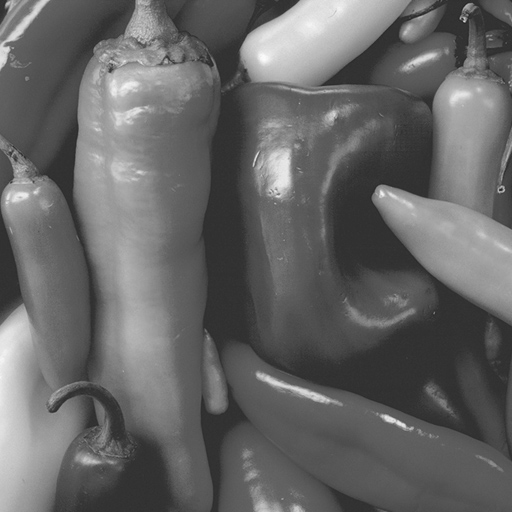
\includegraphics[width=100px]{body/figures/results/blur/input.png}
  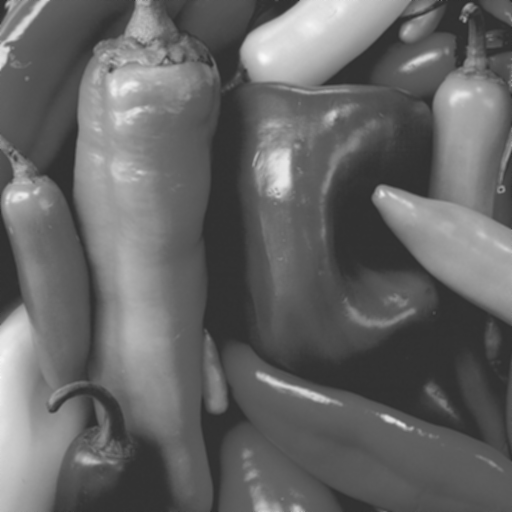
\includegraphics[width=100px]{body/figures/results/blur/cuda.png}
  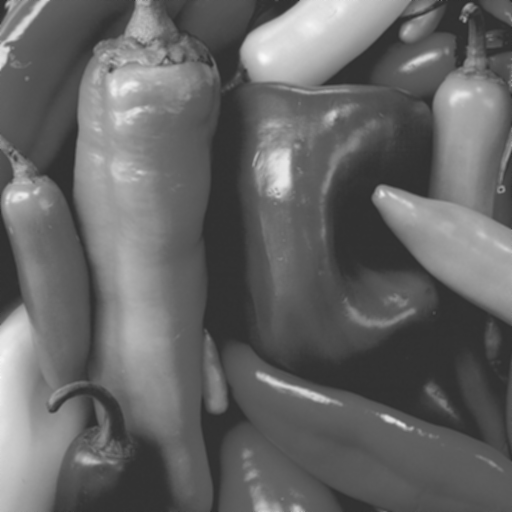
\includegraphics[width=100px]{body/figures/results/blur/julia.png}
  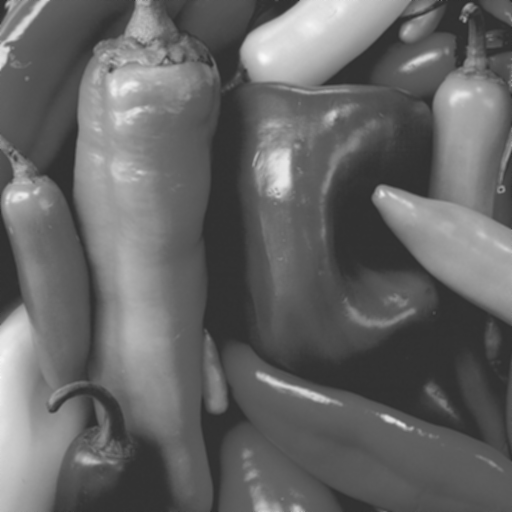
\includegraphics[width=100px]{body/figures/results/blur/opencl.png}
  \caption{Original, CUDA, Julia, OpenCL}
  \label{fig:res:blur:pic}
\end{figure}

By examining the pictures we can see that each implementation has the
same effect on the original image to the left.

### Performace evaluation ###

\begin{figure}[H]
  \begin{center}
  \includegraphics[width=300px]{body/results/blur/total.png}
  \includegraphics[width=200px]{body/results/blur/exec.png}
  \includegraphics[width=200px]{body/results/blur/mem.png}
    \caption{}
    \label{fig:res:blur}
  \end{center}
\end{figure}

## Matrix Multiply ##

The Matrix Multiplication benchmark is a simple $C = A * B$ matrix
mulitplication where $A, B, C$ all are $n*n$ matrices. The benchmark
is executed for all the supported datatypes, 32 and 64 bits integer
and floating point numbers. We here compare the Julia kernel to the
ones produced by OpenCL and CUDA C along with a CPU implementation.
The CPU implementation is simply the matrix multiply operator in the
Julia language.

\begin{figure}[H]
  \centering
  \includegraphics[width=200px]{body/results/mm/int32.png}
  \includegraphics[width=200px]{body/results/mm/int32.png}
  \caption{Int32, Int64}
  \label{fig:res:mm}
\end{figure}

\begin{figure}[H]
  \centering
  \includegraphics[width=200px]{body/results/mm/int32.png}
  \includegraphics[width=200px]{body/results/mm/int32.png}
  \caption{Float32, Float64}
  \label{fig:res:mm}
\end{figure}


\end{markdown}
